\section{Let's Start: Our First Visualisation}
\label{tutorial_03}

\tick{\textbf{Goals:} The objective of this section is to create a first visualisation for an Event-B model of a simple lift system. 
You will learn to create the actual visualisation and to link the visualisation with a formal model by establishing observers.
In addition, you will see how to add interactivity to the visualisation.}

\subsection{Preparing a new Visualisation Template}

The easiest way to create a new visualisation template is to duplicate the default template \texttt{b\_template} that is included in the \texttt{workspace} folder of your \bms~installation.
Just duplicate the \texttt{b\_template} folder and rename it to \texttt{lift}.
After refreshing your browser, it should look like as shown in Figure~\ref{fig_tut_01_workspace}.

\begin{figure}[!ht]
\begin{center}
	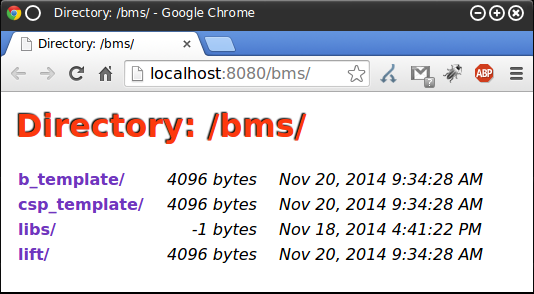
\includegraphics[]{img/tutorial/tut_01.png}
	\caption{\bms~Workspace}
	\label{fig_tut_01_workspace}
\end{center}
\end{figure}

Navigate to the lift folder. The folder contains three files:

\begin{itemize}
\item \texttt{template.html}: This file is the root file of your visualisation. It contains the actual visualisation and it's configuration.
\item \texttt{template.groovy}: The Groovy script file is the place where you can setup your observers.
In particular, the Groovy script file is the link between the formal model and the visualisation.
It allows you to programmatically control the ProB animator and to access the actual formal model being visualised.
You can establish functions that can be called from the visualisation, e.g. executing an Event-B event after pressing a button in the visualisation.
\item \texttt{template.js}: The JavaScript file is needed to initialise your visualisation.
Moreover, it is the starting point to take advantage of the JavaScript language.
There are a lot of libraries for JavaScript that you can apply to create custom visualisations if they have specific needs in a particular domain. 
For instance, libraries exist for manipulating the DOM of an HTML document, or for generating chart and plot diagrams.
In addition, you can call functions that are defined in the Groovy script file.
This enables you to add some interactivity to your visualisation.
For instance, pressing a button in your visualisation could cause the execution of an Event-B event.
\end{itemize}

\subsection{Simple Lift Model}

We are going to create a visualisation for a simple, single lift system that allows movement of a single lift cage between three floors.
The door of the lift can be closed and opened - all in response to the pressing of floor call and cage send buttons.

You can download the corresponding Event-B model \file{EventBLift.zip}{here}.
Decompress it and put the files into a new folder called \texttt{model} relative to your \texttt{template.html} file located in your workspace.
The next step consists of linking the model with the visualisation.
For this, open the \texttt{template.html} with a text editor of your choice and add the line shown in Listing~\ref{lst:htmlmodelline} within the head tag.

\begin{lstlisting}[float=ht,language=html, ,caption={Linking an Event-B model and the visualisation},label=lst:htmlmodelline]
<meta name="bms.model" content="model/MLift.bcm" />
\end{lstlisting}

We link the visualisation with the Event-B machine called ``MLift''.
Linking a formal model within the template file loads the model automatically, whenever you start the visualisation.
Your \texttt{template.html} file should look like in Listing~\ref{lst:htmlmodelline2}.

\begin{lstlisting}[float=ht,language=html, ,caption={Template HTML file after linking the Event-B model with the visualisation},label=lst:htmlmodelline2]
<html>
  <head>
      <title>BMotion Studio for ProB</title>
      <meta name="bms.model" content="model/MLift.bcm" />
      <meta name="bms.tool" content="BAnimation" />
      <meta name="bms.script" content="template.groovy" />
      <script data-main="template" src="/bms/libs/requirejs/require.js"></script>
  </head>
  <body>
  </body>
</html>
\end{lstlisting}

\info{The meta tag \textit{bms.script} contains the link to the Groovy script file and the meta tag \textit{bms.tool} defines the formalism or the simulator respectively that should be used. In this case we are creating a visualisation for a ``BAnimation'' (Classical-B or and Event-B).}

\subsection{Creating a Visualisation}

The user is not restricted to an editor in order to create a visualisation.
The user can make use of any tool that support the creation of SVG graphics or HTML documents.
For this tutorial we are going to use the Inkspace\footnote{\url{https://inkscape.org}} editor. Inkscape is an editor for creating vector graphics that is available for Windows, Mac OS X and Linux.
It's free and open source.
With Inkscape the user can export the vector graphic into the SVG format.

%\info{We are currently working on a build-in graphical editor for creating SVG graphics and for managing observers.}

\begin{figure}[!ht]
\begin{center}
	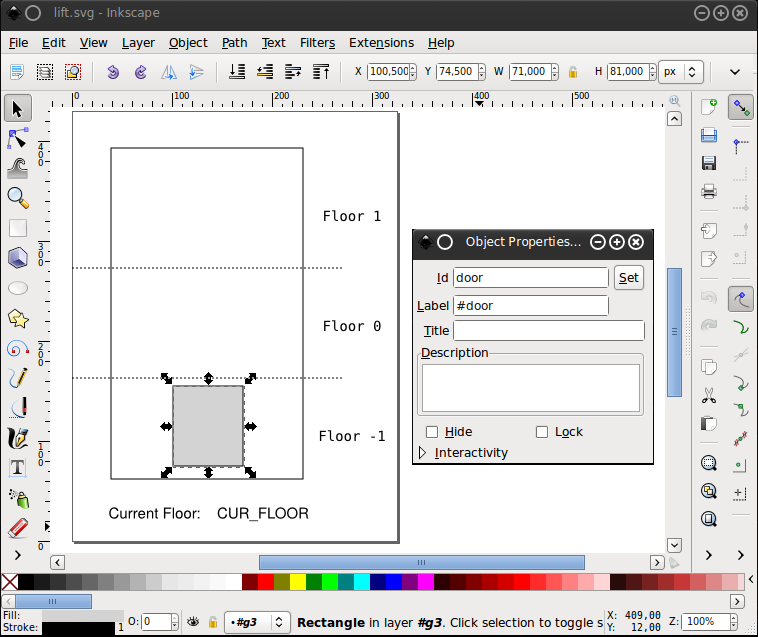
\includegraphics[width=\textwidth]{img/tutorial/tut_02.png}
	\caption{Creating an SVG graphic with Inkscape}
	\label{fig_tut_02_inkscape}
\end{center}
\end{figure}

Please download the prepared \file{lift.svg}{lift.svg} file and open it with Inkscape as demonstrated in Figure~\ref{fig_tut_02_inkscape}.
Feel free to modify and explore the SVG graphic.
In order to link visual elements of the SVG graphic with the formal model, we have to give them identifiers. 
For this, select an element, open the context menu and select \textsf{Object Properties}.
A popup window should be opened as demonstrated in Figure~\ref{fig_tut_02_inkscape}.
As an example, we give the visual element that represents the door, the id ``door''.
In Section~\ref{sec_creation_observers} we explain how we can use this information in order to create the link between the formal model and the visualisation by means of observers.

If you are satisfied with your SVG graphic, save it as a plain SVG graphic with \textsf{File $\rangle$ Save As}.
Select \textsf{Plan SVG (*.svg)} as an output format and click on the \textsf{Save} button.
You can save the SVG file anywhere on your local system. 
Open the SVG file with a text editor of your choice and put the SVG code within the body tag in the \texttt{template.html} file located in your workspace.
Your \texttt{template.html} file should look like in Listing~\ref{lst:lifthtml}.

\begin{lstlisting}[float=ht,language=html, ,caption={Template HTML file with Lift SVG graphic},label=lst:lifthtml]
<html>
  <head>
      <title>BMotion Studio for ProB</title>
      <meta name="bms.model" content="model/MLift.bcm" />
      <meta name="bms.tool" content="BAnimation" />
      <meta name="bms.script" content="template.groovy" />
      <script data-main="template" src="/bms/libs/requirejs/require.js"></script>
  </head>
  <body>
      <svg width="325" height="430" xmlns="http://www.w3.org/2000/svg">
            <rect stroke="#000000" id="svg_1" height="331" width="192" y="37" x="39" fill="#ffffff" />
            <line id="svg_2" y2="267" x2="270" y1="267" x1="0" stroke-dasharray="2,2" stroke="#000000" fill="none" />
            <line id="svg_4" y2="157" x2="270" y1="157" x1="0" stroke-dasharray="2,2" stroke="#000000" fill="none" />
            <rect fill="lightgray" stroke="#000000" x="101" y="275" width="70" height="80" id="door" />
            <text font-weight="normal" xml:space="preserve" text-anchor="middle" font-family="Monospace" font-size="14" id="txt_floor1" y="110" x="280" stroke-dasharray="2,2" stroke-width="0" stroke="#000000" fill="#000000">Floor 1</text>
            <text id="txt_floor0" font-weight="normal" xml:space="preserve" text-anchor="middle" font-family="Monospace" font-size="14" y="220" x="280" stroke-dasharray="2,2" stroke-width="0" stroke="#000000" fill="#000000">Floor 0</text>
            <text id="txt_floor-1" font-weight="normal" xml:space="preserve" text-anchor="middle" font-family="Monospace" font-size="14" y="330" x="280" stroke-dasharray="2,2" stroke-width="0" stroke="#000000" fill="#000000">Floor -1</text>
            <text fill="#000000" stroke="#000" stroke-width="0" x="145" y="407.5" id="txt_cur_floor" font-size="15" font-family="Helvetica, Arial, sans-serif" text-anchor="left" xml:space="preserve">CUR_FLOOR</text>
            <text fill="#000000" stroke="#000" stroke-width="0" x="36.5" y="407.5" id="svg_3" font-size="15" font-family="Helvetica, Arial, sans-serif" text-anchor="left" xml:space="preserve">Current Floor:</text>
    </svg>
  </body>
</html>
\end{lstlisting}

Let's try out the visualisation for the first time.
In your browser, navigate to the \texttt{lift} folder and click on the \texttt{template.html} file.

The visualisation should start.
At the right bottom you will find a menu called \textsf{Open View} for opening different ProB related views.
For instance, Figure~\ref{fig_tut_03_running1} shows the running Lift visualisation with the ProB Events view opened.

At the moment nothing spectacular happens when you change the state (i.e. executing events in the Event view).
In the next Section we are going to create our first observers.

\begin{figure}[!ht]
\begin{center}
	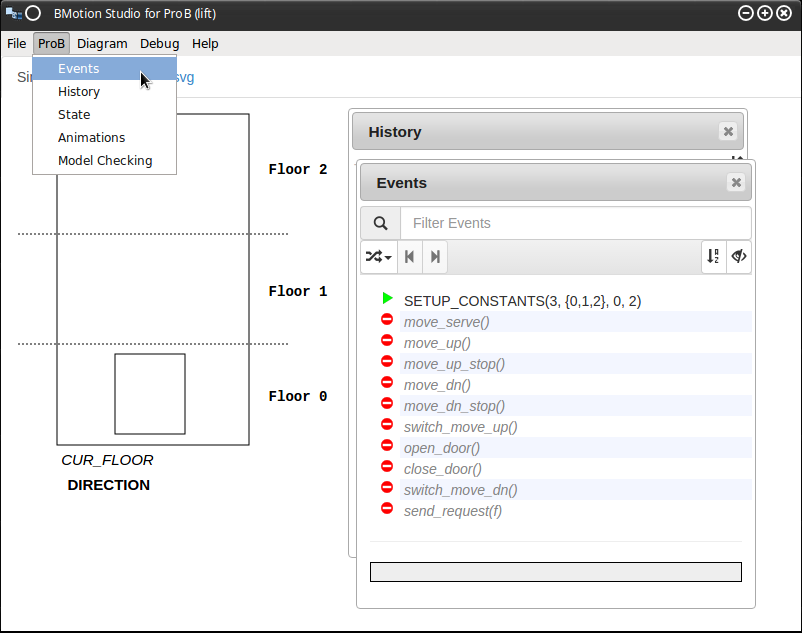
\includegraphics[width=\textwidth]{img/tutorial/tut_03.png}
	\caption{Running the Lift Visualisation for the First Time}
	\label{fig_tut_03_running1}
\end{center}
\end{figure}

\subsection{Creating Observers}
\label{sec_creation_observers}

(tbd)

\subsection{Add Interactivity}

(tbd)

\subsection{Starting the Visualisation}

(tbd)
